\documentclass[a4paper,10pt]{book}
\usepackage[utf8]{inputenc}
\usepackage{graphicx}
\usepackage{hyperref}
\setcounter{tocdepth}{3}

\begin{document}




\section{Abstract}
Approach for potentially high growth services/applications on smart devices (smartphones and tablets).
Theoretical foundations for high growth startups then an approach and an architecture 
In this innovation thesis, we argue for a pretotype architecture for thick client server systems, 
that serves the needs in the first phase of pretotyping and can evolve to a scalable system.


\tableofcontents

\newpage

\section{Introduction}

\subsection{Motivation}
Since Amazon, one of the worlds largest online book stores, launched its Kindle e-Inc reader in 2007, the book market has undergone a big change. 
Millions of people are reading ebooks on different e-Ink readers, smartphones and tablets (denoted \emph{eReaders}) \cite{1}\cite{2}\cite{3}\cite{4}\cite{adultEbookSecondLargestBookFormat}.
In April 2011, ebooks outsold printed books at Amazon for the first time \cite{amazonEbookSurpassedPrint} - and some 
believe this will become true not only for Amazon, 
but for the industry as a whole \cite{barnesEbookPassPrint}\cite{halfPreditEbookDominant2014}.
In other words, we might be witnessing a \emph{disruption}, a total reshaping of the book publishing industry, 
paving the way for great innovation opportunities. 
Companies like Microsoft, Apple and Google are competing for the ebook market \cite{microsoftInvestInNook}, as well as 
several startups \cite{startupEbookChegg}\cite{startupEbookInkling}\cite{startupEbookKno}.


A successful disruption of print books can reach far beyond the publishing industry.

Textbooks are a cornerstone in the education system, and its creation and distribution is the first activity in 
the chain of activities that together constitute the public education's 
\emph{value network} \cite{DisruptingClassExpandedEdition}. A \emph{value network} comprises all activities by different partners, 
suppliers and channels that together serve particular customers.

The US education system is becoming too expensive \cite{theInnovativeUniversity}. 
With continuously increasing tuition fees \cite{risingTuitionFees}\cite{theInnovativeUniversity} and student debt 
reaching a staggering 1 trillion USD in the US \cite{oneTrillionUsStudentDebt}, the education market is in need of 
more affordable alternatives. Combined with a fundamental mismatch between the unique individual student learning 
preferences and the increased standardized of education \cite{DisruptingClassExpandedEdition}\cite{educationInnovationNecessaryForEconomicGrowth}, 
the education industry is itself ready for disruption \cite{DisruptingClassExpandedEdition}\cite{theInnovativeUniversity}.

Indeed, the disruption might already have started. In recent years, online course enrollment in the US has increased 
"substantially faster than overall higher education enrollments" \cite{babsonOnlineEduGrowth2011}. Specifically, online 
enrollments growth rate has been more than ten times the growth rate of overall higher education enrollments in the fall 2010. 
31 percent of all higher education 
students take at least  one course online, and 67 percent of academic leaders rated the learning outcomes 
"as the same or superior to those in face-to-face" \cite{babsonOnlineEduGrowth2011}. 
Clayton M. Christensen, a leading expert in disruptive innovation theory, predicts that by 2019,
fifty percent of all high school courses will be delivered online \cite{DisruptingClassExpandedEdition}.

However, a disruptive online education, or more generally computer-based learning, is not a mere replication of the monolithic 
"bricks and mortar" education online \cite{DisruptingClassExpandedEdition}. Despite heavy investment in computer systems, previous attempts have 
largely failed to deliver significant improvements, because the technology has been co-opted to the existing teaching model, serving 
existing students \cite{DisruptingClassExpandedEdition}. 
Instead, to be successful, a new student-centric teaching model ducational system 
about using a new tool to deliver the same monolithic experience, 
but rather
There are interesting innovations in online education, including Coursera's Massive Open Online Courses (MOOC), some of which 
and khan translated to more than 50+ languages. It is appealing to an international audience (not just the US).
Education is competitiveness, 
With a global education spending of 4 trillions USD per year predicted to double by 2020 to 8 trillions USD...
In this innovation thesis, I am initially asked by a startup to build an eReader application for Android. With this fast paced ebook and educational market,
ambitions quickly got higher - eReaders are more than books. Not only digitize the reader. Interconnected, powerful devices.
However, startups fail, and even established companies.

So, need learn big picture, deduce requirements for process and architecture.

Many educational startups emerged in recent years \cite{boomEducation1}\cite{boomEducation2}, as well as big players like Apple, Intel, 
Google and Microsoft battling for the education market. The estimated global spending on education is about 4 trillion USD, projected to grow to
8 trillions USD by 2020.

Massive Open Online Courses (MOOC), courses with large scale student participation from few thousands to hundreds of thousands of participant 
in a given course.


Nation competitiveness. But not standardized, customized, user sharing etc.

... while agile project requirement collection is important and done with an existing customer, innovation 
has no defined customer. Needs to be found, defined and needs met.
So, understanding innovation, entrepreneurship etc. is a kind of requirements collection.

\section{Background}
\subsection{The tablets, smartphone and ebooks rise}
Publishing / book industry shifting
\\
Google 1.3 million device activated per day; each one seems to be new device, no upgrade ...
\\ 
Apple sold more tablets than any other PC manufacturer sold laptops
\\
“The increasing consumption of digital content has primed the textbook market for disruption, 
creating an exciting opportunity for technology innovation to fundamentally change the way 
1.4 billion students globally learn,” Arvind Sodhani, president of Intel Capital, said in the statement.

http://www.businessweek.com/news/2011-04-08/intel-capital-leads-30-million-funding-of-education-startup-kno.html

eReaders and tablets: disrupting books?
tablets: disruptive technology to disrupt even further industries?
\\
Big opportunity

\newpage
\subsection{Disruptive Innovation: understand what is happening}
In a given market, customers have needs, or \emph{jobs-to-be-done} \cite{DisruptingClassExpandedEdition},
addressed by a process, service or product (subsequently \emph{product} for short) \cite{scientificArticlePredictingTheUnpredictable}.
Customers value a product's performance along different characteristics, some of which are \emph{drivers}, i.e. 
the most important when selecting a product. For a given driver, different customers have different sophistication levels. 
Customers at the \emph{low-end} can be satisfied with 
less sophistication and performance, while customers at the \emph{high-end} are interested in more performance \cite{innovatorsSolution}. 

For example, a low-end customer for a computing device for gaming might be satisfied with an average performance (CPU, memory, graphics card etc.), 
while a high-end customer might want top performance and looks up for the next performance improvements.

Usually, profit margins, the percentage of profit out of the total sale, are higher at the high-end of the market than the low-end, thus 
making it more attractive.
To stay competitive, companies continuously make \emph{sustaining innovations} to improve their products, enabling them to serve more and more of 
the high-end customer needs. For example, a more performant graphics cards. This is depicted in Figure \ref{fig:disruptiveInnovationModel}.\\

\begin{figure}[here]
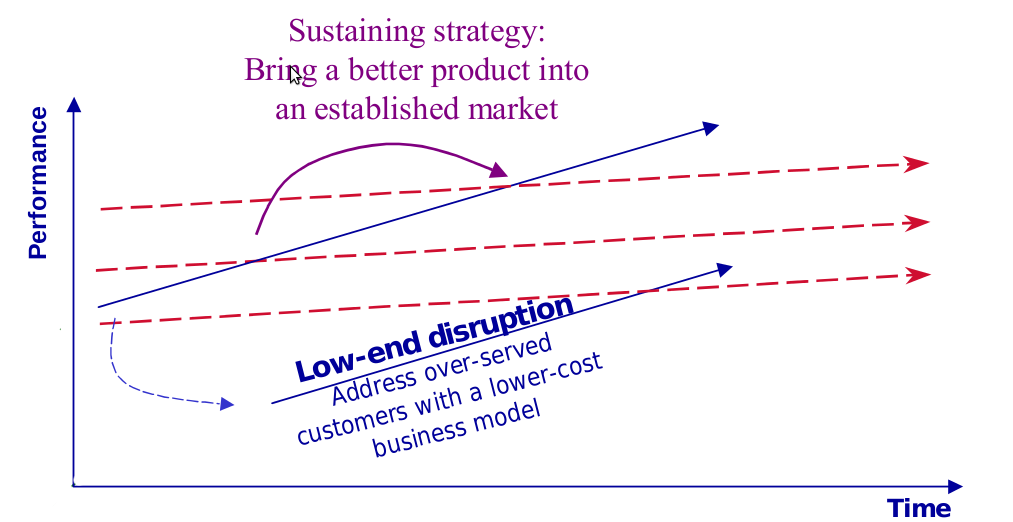
\includegraphics[width=0.9\textwidth]{images/simpleDisruptiveInnovationModel.png}
%\includegraphics{new_look_contents.png}
 \caption{The Disruptive Innovation Model (source: \cite{innovatorsSolution})}
\label{fig:disruptiveInnovationModel}
\end{figure}

The upper blue arrow represents the product performance growth over time. The sustaining innovations improve 
the product's "attributes most valued by the industry's mainstream customers" \cite{innovatorsSolution}, i.e. the drivers. 

However, according to the disruptive innovation theory, the pace at which companies improve their products by sustaining innovations is faster than 
the growth of customer sophistication - the ability to utilise or absorb improvements. 
This is illustrated by the stippled red lines in figure \ref{fig:disruptiveInnovationModel}. For example, a graphics card performance improvements
beyond what is sufficient to play less demanding games does not effect low-end or casual gamers.

Over time, more and more customers become \emph{overserved}. The product becomes more complex and costly without valuable leverage for most customers. 
Despite this trend, the established company tend to continue doing what it has been optimized over the years to do: sustaining innovations.
The company has built internal and external structures that are optimized for competing in the high-end market, 
including its vision, processes, policies, assets, valued competencies, corporate culture \cite{scientificArticlePredictingTheUnpredictable}, 
as well as its \emph{value networks} \cite{innovatorsDilemma}.
A value network is "the collection of upstream suppliers, downstream channels to market, 
  and ancillary providers that support a common business model within an industry." \cite{innovatorsDilemma}. 
That is, all its relationships and integrated processes with partners within the market.
This solidifies its position in the current market against any new entrant (e.i. startups), 
but at the same time makes it vulnerable for changes in the market, including changes in the priority of the dominant drivers.


This opens the door for \emph{disruptive innovations}, typically done by new entrants (i.e. startups) into the market with a new business model 
that can change the market significantly. \\

There are two types of disruptions, \emph{low-end} and \emph{new-market disruptions}, depending on the initial target customers.

In low-end disruptions, an entrant company starts by offering a product that is good \emph{enough} to the existing low-end market in regard
to the dominant driver, using a business model that enables profits at lower prices. 
Furthermore, the product might be better in regard to other characteristics as simplicity and convenience \cite{innovatorsSolution} 
making it a better choice.
This is illustrated by the lower blue arrow in figure \ref{fig:disruptiveInnovationModel}.

The disruptor company is built around a new business model better suited for the low-end, which gives it the advantage.  
Instead of fighting back, the established company tend to abandon the unattractive low-end and focus on the more attractive high-end market, where it has
a competitive advantage. In the short term, this is more profitable, "feels good" and makes "perfect sense" \cite{innovatorsSolution}. 
Thus, the established companies ignore the eminent threat. 
However, as the disruptor begins its own cycle of sustaining innovations, it gradually improves the product in regard of the dominant driver 
and builds its value network to serve more needs in the high-end, 
thereby pushing the established companies upward in the market. 
This continues until the bulk of customers are 
attracted to the new entrant company, thereby disrupting the market. Because the bulk of the customers are usually concentrated in the 
middle of the sophistication scale, when the disruptor matures enough for the mainstream customers this results in a relatively 
quick and sudden market change. The old companies are either reduced to the high-end niche or disappear completely.


On the other hand, in a new-market disruption, the disruptor starts by offering 
typically a simpler, more convenient product to \emph{nonconsumers}.
Nonconsumers are persons that previously either could not afford or did not have the skills to use the products in the established 
market.
Thus, the new entrant company competes against "non-consumption", by offering a product to a whole new population that have no alternative. 
This type of disruption is the most frequent \cite{disruptionInEducation}. \\
This is illustrated in figure \ref{fig:twoDisruptiveInnovationModels} by a new (green) plan.

\begin{figure}[here]
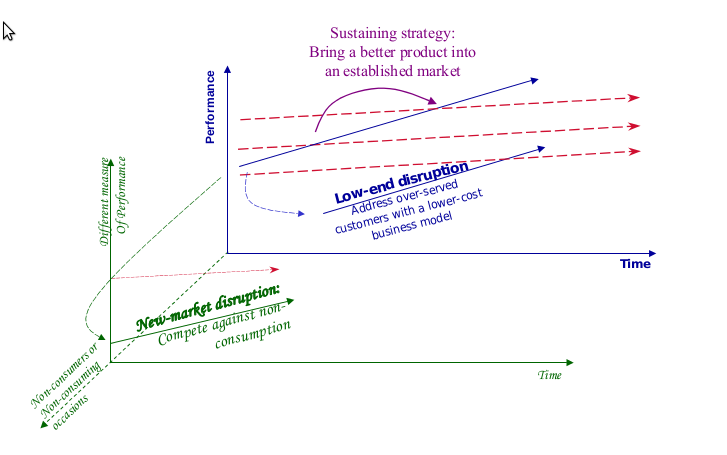
\includegraphics[width=0.9\textwidth]{images/twoDiruptiveInnovationModels.png}
%\includegraphics{new_look_contents.png}
 \caption{The Two Disruptive Innovation Models (source: \cite{innovatorsSolution})}
\label{fig:twoDisruptiveInnovationModels}
\end{figure}

Initially, the product is not sophisticated enough for the existing customers in the old market, 
and the performance is perceived differently in the new market. However, as in the case of low-end disruptions, the product improves
gradually and eventually pulls customers from the old to the new market.\\

Employing disruptive strategies, both low-end, new-market or a combination, many companies accross different industries 
have successfully overtaken markets \cite{innovatorsSolution}. For instance, when the Apple II computer was launched, it was too basic 
for the financial and engineering applications that used to be handled by minicomputers. Apple II was sold as "children's toy" thereby 
creating a whole new market that previously did not exist \cite{disruptionInEducation}. 
As personal computers improved, they disrupted the minicomputer market. 

Most successful disruptions have three enablers: 
a simplifying technology (makes it simpler and/or more convenient to do a job etc.), a business model innovation (who are the customers, 
what value proposition to offer, key processes and resources, and a profit formula \cite{reinvetingBusinessModel}), and a new disruptive 
value network \cite{pressArticleHbsReviveHealthCareInnovation}. A disruptor rarely disrupts the market alone, but an entire new value 
network arises that replaces the old one \cite{DisruptingClassExpandedEdition}\cite{pressArticleHbsReviveHealthCareInnovation}. 




Link to effectuation
"Therefore, there is a good reason to speculate
that the entrepreneurship literature may offer contributions to advance the disruptive innovation
research and offer valuable guidance to managers. However, as shown in the table, to-date the direct
linkage between the two streams of research has been minimal." \cite{managingDisruptiveInnovation}



Link effectuation: weak:

"Second, effectuation typically only works for evolutionary development, while for
radical disruptive innovations the causation model is more appropriate. Since the effectuation
model starts from what is already there and gradually develops this into something new, it
hinders the development of revolutionary changes. For such changes, vision, long term goals,
anticipation of customer needs, and thinking beyond what is currently possible are important
(Walsh, 2004). Hence, both the effectuation and the causation models can be suitable for the
development and creation of new products and markets." \cite{}

"New Technology-Based Firms in the New Millenium", Chapter 13:  The Nature of the Entrepreneurial Process: Causation, Effectuation, and Pragmatism



"Exaptation process is more effective in generating disruptive innovation than adaptation
process"  \cite{managingDisruptiveInnovation}
Exaptation: "a feature co-opted for its present role for new purposes but not an adaptation for its
current function"

TATA: not known, can target a given market and end elsewhere.

"Predicting which artifacts or design will turn into the next disruptive innovation is not an easy task
due to the presence of Knightian uncertainty (unknown and unknowable conditions) of plausible
product/design features combinations and permutations. "


"Lead user innovation is an effective approach for leveraging outsiders and tap into their innovative
ideas. Although the literature tends to report only the incremental innovation potential of lead users,
we argue that the literature has overlooked the lead users such as the founders of Facebook, ..."

TATA: engage the users, partnership. Forums?

" can leverage the communities of users of their products and learn to distinguish and
reward top ideas and artifacts through company-based initiatives or even leveraging external online
platforms that focus on this."




\begin{enumerate}
 \item Forget products/market segments, it is all about jobs-to-be-done: the roots why people "hire" a product
 \item "People don’t want a quarter-inch drill—they want a quarter-inch hole."
 \item Sophistication of customer needs (jobs-to-be-done) grows slower than technology advancement 
 \item Technology breakthrough almost irrelevant in and by itself
 \item Disruption starts either at the low end or non-consumers (can't afford/too complicated etc.) - low tech/low capacity/can do less
 \item But makes it easier, more accessible and/or more affordable
 \item High end companies shift focus to more sophisticated markets, quality and high margines; makes sense and feels good
 \item Disruptive innovators get better and better, until technology advancement satisfies more and more jobs-to-be-done
 \item Traditional companies collapse
 \item Due to residuents in established companies, and the requirement to adjust the whole organization to satisfy the job-to-be-done from ground up
  established companies rarely succeed in disruptive innovations. They are adviced to create a separate startup like unit.
\end{enumerate}

 - understanding jobs to be done is the starting point, build everything upon it

Findings applied to education 
(Note: IT disrupting education, not only iPads. But iPads/eReaders disrupting books -> disrupting textbooks used in education?)
\begin{enumerate}
 \item Traditional way of education is too inflexible, standardized, students run in batches, subjects and departments are silos
 \item People learn differently, different paces, different interests and capabilities 
 \item Learning best by creating and engagement two-ways or peer-to-peer, not one-way-hearing \cite{disruptiveOrLiberatingEducation}
 \item Creativity comes at cross-roads of different disciplines 
 \item " ...schools.. online learning programs failed simply because they tried “to provide traditional courses in a nontraditional manner.”"
 \item " Attempting to market an inferior product to their most demanding customers was, predictably, a recipe for failure"
 \item "...problem was that they were still competing against consumption."
 \item is ready for disruption
\end{enumerate}


-----------
Rita Kop, “Web 2.0 Technologies: Disruptive or Liberating for Adult Education?” Adult Education Research Conference 2008, St. Louis, Missouri, June 5–7, 2008.

Students need to create content, get it validated by peer (Tayeb: voting?) and expert feedback.
Free to construct, but get validated instead of one-way-hearing. Maybe not fully understand until validating ones own thoughts?
Get knowledge from different sources, no time/space limits. Chaos, creativity.

"... people take ownership of the learning process, rather than institutions controlling their education"

"... they preferred the online
mode of study, which is flexible and available at the time and place to suit them and fitting in
with their lifestyles better than face to face teaching, [but] they required a lot more nurturing than
anticipated. "
-----------

conclusion:?
Courses with lots of books, deep\\
Non-consumers(non-students): Books, "randomly chosen", by topic, on your own.\\
Offer: Package mini courses with the books in one package, peer-to-peer.!
\\
But how do expert do it?

Genome:
"...large companies are excellent at sustaining
innovation but by and large fail at disruptive innovation. Startups thrive on
creating disruptive innovations. Recently, thought leaders in entrepreneurship
have come to the conclusion that in order for large companies to be effective at
disruptive innovation they need to make structural changes that make them
behave nearly identically to startups."

\subsection{Expert Entrepreneurs Effectuation}
No stubburn long term vision - but adapt and in partnership build the unforeseeable future.
 - no initial clear-cut idea.

\begin{enumerate}
 \item Bird in hand (arabic books, understand language and culture, network) - and find and do what is doable.
 \item Affordable loss
 \item Partnership - then find partners to work together and reshape goals if necessary (now move to k12 with iqra school instead of university-wish-to-be)
 \item Leverage surprises (Use uncertainty to own benefit)
 \item Pilot in the plane (future made, not predicted)
\end{enumerate}

It specific?
 
So, how expert entrepreneurs are doing it?
 - the venture is shaped 
 
 
\subsection{Holding balance: Organic Startup Dimensions, morph into big company}
A startup anology that works well, is organ development in early stages. 
Need to grow harmoneously between all ingredients/dimensions of startup, until it reaches a final shape;
And find itself/identity to form and adapt to how to serve a specific need/market-to-be.
Then it can grow on this foundation.

According to Genome types, Padness is "The Social Transformer / Type 1N" (social reading/studying)

So, as Disruptive Innovation sais about jobtobedone and forge the whole based upon, organ has to form itself. Ok

Findings:
"Startups need 2-3 times longer to validate their market than most founders
expect. This underestimation creates the pressure to scale prematurely"

"Startups are temporary organizations designed to scale into large companies.
Early stage startups are designed to search for product/market fit under
conditions of extreme uncertainty. Late stage startups are designed to search for
a repeatable and scalable business model and then scale into large companies
designed to execute under conditions of high certainty."

The Organic Startup
 How should IT-startups do it? Jobs-to-be-done is discovered and startup builds around it and a business model, and grow organically
 to be a grown up company.
 A balance excercice between all aspects of the startup
 

\subsection{Pretotyping}
Matches great, and the Agile movement/Lean startup
Early stage: pretotyping find the job(s) to be done
\\
Interpretation: shorten the speculative phase and back it up with user data
\begin{enumerate}
\item iteration, 
\item AB test, Google made millions of \$ on changing link blue color shades to figure best.
\item data collection, 
\item metrics, 
\item one or more projects
\item Continuous deployment
\item First disable caching, to get most hits, then enable if necessary
\end{enumerate}

Small AB tests, too much to require users to install and reinstall different
Early stage development: Minimum Viable Product pretotyping
 - What pretotyping is
  --- beware vanila metrics, i.e. user growth if no revenue stream.
 - beta, alpha
 - AB/split test
 - Requires Quick development/deployment
 



\subsubsection{Challenges of pretotyping on thick clients}
To be Quick is fine, but needs flexibility to change. However, backward compatibility imposed, delays might incur etc.
Needs to reverse quick bad decisions. Keep control over architecture (well behaved clients).
 * Challenges of thick client pretotyping
 - Client distribution out of control: external distributor. Sometimes restrictions/rejection, delays in distributing update etc.
 - unflexible for pretotyping practice (cons)
    - For example if one makes a quick pretotype with heavy polling, then it shows to be too much, not possible to easily retire the client.
   not easy AB test: no full control over installs. 
 - In beginning, important to convey a good image and make to be a "sticky" app in the users mind. Before that, don't annoy/expect user
   with too many re-installs
 - Forced external API Design (cons but make it advantage - prepare platform API, and possible easier partnership)
    API deprecation, reverse wrong design: keep control over system
 - Architecture: 
    Cost and difficulty when time passes, for website, even more when no control over a component in the architecture:
      change in Design --costs(++)--> Impl.
      scala+perf. most difficult to adjust. Anecdote: Amazon split server for Christmas season. Might have had significant concequences.
    performance, scalability and reliability (advantage thick client computation available)


Communication with users
AB test

\subsubsection{public API trend, and platform a good way to go}
A public API is a way to build an eco system around a product/service, it is a trend and should be envisaged.
However, API's as stars in the universe, inchangeable and will be wrong first time.
Prepare for evolution, deprecation.
So, my own note: use it internally before public, eat you own food.

\subsection{Architecture}
Although probability low, and many focus on scalability too early, bad if chance goes away and we are here for high growth systems anyway.
So, make lightweight decisions that keep my system open for scalable solutions in the future with relatively small price.

Keep all possibilities open, open evolvable architecture for different loads.
\begin{enumerate}
\item Design costs less, after costs more...
\item Scalability and performance are most difficult to add as an afterthought
\item An architecture that both satisfies the needs of the pretotype in early stage, but can evolve
    into a scalable solution
\item QRCS read-write separation
\end{enumerate}

Client loadbalancing.
Cloud more expensive than own. Cloud not good at scalability; cannot optimize (commodity), [not near CPU, LMAX architecture,...].
Plus, cost saving in beginning important. Investment postponed, but success needs most of hardware investment, so best:
Client load balancing, hybrid cloud-hosting.

\section{Approach}
A (3osarat) resume is to:
- start from what one have: I am arab, student, know educators and publishing houses in arab world, have access to copyright free books
- niche good, focus.
- build basic seed add what opens different types of partnerships: investors (collect data, but disable if too much), authors (feedback), 
self-authors (+corrections), schools (teacher<->students<->students), publishers (correction, usage stats), software houses cooperation.

--- in the light of education disruption

- make lightweight architecture (remote control, API Design, scalability if it comes)
-- separate client from server, enable each to evolve 
-- separate backend by two dimensions: 1) services, 2) read-write
- launch then look for partnerships with concrete product and user numbers (more credibility with product in hand)
- Hold eye on growth: if scale, move to arch, otherwise optimize user experience, user retention, feedback loops etc. until it takes off.
- continuous integration/deployment, test. However, might be too complicated if simple backend, introduce when necessary.


\section{Case}
\subsection{Use cases}
\begin{enumerate}
\item Easy corrections
\item Class mate and group reading
\item Asking clarifications from author
\item Author understanding of book unclear passages, reading patterns etc. to improve book
\item Author More data about how book is read, time spent etc.
\end{enumerate}
 
 IDEAs: 
 - ebooks that change depending on type of user learning preferences (?)
 - MEAP/Manning: books dev-loop and sold. What about more dynamic, realtime feedback loop?
 

\subsection{Why/strategy}

 Arabic Niche, Low cmompetition, hope for higher interaction
 iOS success, demand for android

\subsection{Possible paths and what should be done in each case}
If high growth, move to scalable
If low growth, work on customer aquisition and retention
Enhance existing functionality
Add functionality 

\subsection{What happened}
Pretotype with HTML5 (titanium), made book scanner. However too slow.
Some big companies that used it, moved away from it.


In beginning, a thought of developing API, let existing iOS app be enhanced with interaction to get feedback quickly, start immediate iteration
However, problems with external devs, genome sais it!
Dropped and moved to android

Web (minimum), failed, parked
Android: basic has to be in place, pretotype only on new extra features. Challenge


Need fast desicion, product owner present or autonomy.
Authority to decide

\subsubsection{Implementation}
\subsubsection{Arabic}
Arabic letters different forms. Needs reshape. Had an open source starting point, but had bugs for some letters, and no "tashkeel".
Bug long lines, sometimes letters inversed.
Need to estimate line length and cut.

Search: trade off, between size, speed and batteri. Chose speed and batteri - space can be purchased.
word reshaped before indexed - remove tashkeel.


\subsubsection{Log analysis}

\begin{enumerate}
\item Although arguably less user friendly, number of user contents available per page is not available. Interested users would click on it, so
we register interest even if most books have no annotations in the beginnning. Not enough resources to enter/sponsor/encourage initial user 
content.
\item various books different interests, too scattered user annotations. To get momentum, needs focus user groups, for example cooperate on 
particular course and get students to interact with each other and teacher through app to add content. Otherwise, users are disappointed.
\item Remarked same users click on different pages from same book, guess frustrating, especially when most have no content, 
so made change added different categories: page, chapter and book.
\item Quite few users attempted repeatedly to login but failed, even after successful registration with arabic names. A bug hindered UTF8 
usernames from client side. Was too cumbersome to fix with time limit. Others tried with email. Quick fix was to send message, 
meanwhile made stricter client validation: no arabic, no email.
\item Quite few failed registration because of weak password. The numbers were quite significant, and turned out they used numbers only password.
Restriction was removed.
\item In general, we need a much easier user account creation and login process, possibly with auto picking user (Google) email if available
and generating a password so user only needs to approve.
\end{enumerate}

\subsection{Requirement and architecture}
Prepare for scalability, even not implementing:
\begin{enumerate}
\item Avoid bottleneck on id generator
\item Shard-able ID creation, one per book well defined algorithm
\item Scalability and performance are most difficult to add as an afterthought
\item An architecture that both satisfies the needs of the pretotype in early stage, but can evolve
    into a scalable solution
\end{enumerate}


\section{Conclusion}


\begin{thebibliography}{9}


%@article{christensen2003disruption,
%  title={Disruption in education},
%%  author={Christensen, C.M. and Aaron, S. and Clark, W.},
%  journal={Educause Review},
%%  volume={38},
%  pages={44--55},
%  year={2003},
%  publisher={EDUCAUSE}
%}

%)

\bibitem{disruptiveOrLiberatingEducation}
  Rita Kop, \\
  “Web 2.0 Technologies: Disruptive or Liberating for Adult Education?” \\
  Adult Education Research Conference 2008, \\
  St. Louis, Missouri, June 5–7, 2008.

\bibitem{innovatorsSolution}
   Clayton M. Christensen, Michael E. Raynor,\\
   \emph{The Innovator's Solution: Creating and Sustaining Successful Growth},\\
   September 2003 \\
   Harvard Business School Press\\
 
\bibitem{disruptionInEducation}
   Clayton M. Christensen, Sally Aaron, William Clark\\
   \emph{Disruption In Education}\\
    2001\\
   \url{http://www.educause.edu/Resources/DisruptioninEducation/158712}\\

    
\bibitem{DisruptingClassExpandedEdition}
   Clayton M. Christensen, Curtis Johnson, Michael B. Horn\\
   \emph{Disrupting Class, How disruptive innovation will change the way the world learns, Expanded Edition}\\
    May 14, 2008\\
    Mc Graw Hill\\

\bibitem{articleDisruptingTextbooksInHigherEducation}
  Disrupting Tree-Textbooks in Higher Education\\
  Daniel Falabella, Salvael Estrada\\
  \url{http://byuia.com/innovation-and-the-academy/}\\
   (Accessed 22 December 2012)

\bibitem{scientificArticlePredictingTheUnpredictable}
  \emph{PREDICTING THE “UNPREDICTABLE”\\
  ANTICIPATING DISRUPTIVE INNOVATION}
  Jay Paap and Ralph Katz\\
  Research-Technology Management, 2004\\ 


\bibitem{onePointThreeMillionAndroidDeviceActivationPerDay}
  Eric Schmidt: “There Are Now 1.3 Million Android Device Activations Per Day”
  %\url{	
   http://techcrunch.com/2012/09/05/eric-schmidt-there-are-now-1-3-million-android-device-activations-per-day/
   %}\\
   (Accessed 15 December 2012)

\bibitem{risingTuitionFees}
 \emph{Tuition Rising: Why College Costs So Much} \\ 
 R. G. Ehrenberg\\
 Harvard University Press, 2002.
 
\bibitem{reinvetingBusinessModel} 
  \emph{Reinventing Your Business Model} \\
  Clayton M. Christensen, Mark W. Johnson, Henning Kagermann\\
  Harvard Business Review, 2009\\
 
\bibitem{theInnovativeUniversity}
 The Innovative University \\
 Changing the DNA of Higher Education From the Inside Out \\
 Clayton M. Christmas, Henry J. Eyring
 Jossey-Bass, 2010
 
 \bibitem{oneTrillionUsStudentDebt}
  %\url{	
 http://www.bbc.co.uk/news/business-20663550
   %}\\
 (Accessed 17 December 2012)

\bibitem{pressArticleHbsReviveHealthCareInnovation}
  \emph{How to Revive Health-Care Innovation}\\
  \url{http://hbswk.hbs.edu/item/6095.html}\\
  (Accessed 23 December, 2012)\\
 

\bibitem{pressArticleIpadDisruptingPcAndGaming}
IPad, tablets clearly disrupting PC market, survey finds\\
\url{http://bgr.com/2011/04/12/ipad-tablets-clearly-disrupting-pc-market-survey-finds/}\\
  (Accessed 23 December, 2012)\\
 
\bibitem{babsonOnlineEduGrowth2011}
  \emph{Going the Distance: Online Education in the United States 2011}\\
  I. Elaine Allen and Jeff Seaman\\
  BABSON Survey Research Group\\

\bibitem{boomEducation1}  
  \emph{Boom time for higher education startups}\\ 
  July 26, 2012,\\
  \url{http://www.oregonbusiness.com/linda/7830-online-higher-education-startups-boom}\\
  (Accessed 21 December, 2012)\\

\bibitem{boomEducation2}  
  \emph{Anticipating a Blended Classroom Boom Led by Education Startups}\\ 
  August 31, 2012,\\
  \url{  http://techcrunch.com/2012/08/31/blended-classroom-boom-education-startups/}\\
  (Accessed 21 December, 2012)\\

\bibitem{courseraTedTalk}
What we're learning from online education \\
Daphne Koller\\
\url{http://www.ted.com/talks/daphne_koller_what_we_re_learning_from_online_education.html}\\
  (Accessed 21 December 2012)

 \bibitem{microsoftInvestInNook}
   \emph{Microsoft Hooks Onto Nook}\\
   \url{http://online.wsj.com/article/SB10001424052702303916904577375502392129654.html}\\
   (Accessed 21 December 2012)
   
 \bibitem{subtextGoogleInvested}
 \emph{Subtext Raises \$3 Million From Google Ventures \& More To Make eBook Reading Social}\\
 \url{http://techcrunch.com/2011/10/25/subtext-raises-3-million-from-google-ventures-more-to-make-ebook-reading-social/}\\
   (Accessed 21 December 2012)
 
 \bibitem{rethinkBooks}
  \emph{Rethink Books Gives Us A Glimpse At Social Books (Video Demo)}\\
  \url{http://techcrunch.com/2010/11/11/rethink-books-social/}\\
  (Accessed 21 December 2012)
  
 \bibitem{startupEbookInkling} 
   \emph{Inkling raises \$17 million – Swings for the Fences}\\
   \url{http://www.edukwest.com/inkling-raises-17-million-swings-for-the-fences/}\\
 (Accessed 21 December 2012)
 
 \bibitem{startupEbookChegg}
   \emph{Chegg eTextbook Reader launches today – Works on any Device}\\
   \url{http://www.edukwest.com/chegg-etextbook-reader-launches-today-works-on-any-device/}\\
 (Accessed 21 December 2012)
 
 \bibitem{startupEbookKno}
   \emph{Intel Capital Leads \$30 Million Funding of Education Startup Kno}\\
   \url{http://www.bloomberg.com/news/2011-04-08/intel-is-said-to-lead-30-million-funding-of-education-tablet-startup-kno.html}\\
  (Accessed 21 December 2012)
   
 \bibitem{nytimesAmazonEbookSurpassedPrint}
  \emph{E-Books Outsell Print Books at Amazon}\\ 
  May 19, 2011,\\
  \url{http://www.nytimes.com/2011/05/20/technology/20amazon.html}\\
  (Accessed 19 March, 2012)\\

\bibitem{adultEbookSecondLargestBookFormat}
   \emph{Trade Sales Rose 13\% in January-June Period, AAP Says } \\
  \url{http://www.publishersweekly.com/pw/by-topic/industry-news/financial-reporting/article/54372-trade-sales-rose-13-in-january-june-period-aap-says.html}\\
  (Accessed 17 December, 2012)\\
  

  \bibitem{1}
   \emph{eBook Market Exploding, Confirms New IDPF Survey}\\
   \url{http://www.huffingtonpost.com/mark-coker/ebook-market-exploding-co_b_507107.html}\\
  (Accessed 19 March, 2012)\\

\bibitem{2}
   \emph{Why E-Books are Hot and Getting Hotter}\\
  \url{http://www.huffingtonpost.com/mark-coker/why-e-books-are-hot-and-g_b_320986.html}\\
 (Accessed 19 March, 2012)\\

\bibitem{3}
   According to the following iTunes stats, 20 percent + of active applications are either books or education related \\
   \emph{App Store Metrics}\\
   (Page last updated: 2012-02-13 06:00:09 -0800 PST): \\
   \url{http://148apps.biz/app-store-metrics/?mpage=catcount} \\
  (Accessed 19 March, 2012)\\
 
\bibitem{4}
   \emph{The Rise and Rise of e-Textbooks [Infographic]}\\
   \url{http://www.getelastic.com/the-rise-and-rise-of-e-textbooks-infographic/}\\
  (Accessed 19 March, 2012)\\

\bibitem{amazonEbookSurpassedPrint}
  \emph{That Was Fast: Amazon's Kindle Ebook Sales Surpass Print (It Only Took Four Years)}\\
  \url{http://techcrunch.com/2011/05/19/that-was-fast-amazons-kindle-ebook-sales-surpass-print-it-only-took-four-years/}\\
  (Accessed 20 March, 2012)\\




\bibitem{barnesEbookPassPrint}
  \emph{Barnes \& Noble: eBooks will pass print -- fast}\\
  \url{http://tech.fortune.cnn.com/2011/03/25/barnes-noble-ebooks-will-pass-print-in-2-years/}\\
  (Accessed 20 March, 2012)\\


  \bibitem{appleITunes300mDownloads2010}
  \emph{iTunes U Downloads Top 300 Millions}\\
  \url{http://www.apple.com/pr/library/2010/08/24iTunes-U-Downloads-Top-300-Million.html}\\
  (Accessed 17 December 2012)

\bibitem{managingDisruptiveInnovation} 
Yanto Chandra , Shu-Jung Sunny Yang
Managing Distruptive Innovation: \\ 
ENTREPRENEURIAL STRATEGIES AND TOURNAMENTS FOR CORPORATE LONGEVITY\\
(Forthcoming in Journal of General Management) \\
Journal of General Management, 37(2): 23-50.\\
2011\\
\url{http://papers.ssrn.com/sol3/papers.cfm?abstract_id=1965000}\\
(Accessed 18 December 2012)

\bibitem{billionTweetsPerTwoDaysAndHalf}
Twitter CEO Dick Costolo: Users Can Download Their Entire Archive By Year-End; Now Sees 1B Tweets Every 2.5 Days \\
\url{http://techcrunch.com/2012/11/26/twitter-ceo-dick-costolo-twitter-sees-a-billion-tweets-every-two-and-a-half-days-users-can-download-their-entire-archive-by-year-end/}\\

\bibitem{amazonDisruptionUnforldingTimothy}
Strategic Disruption, Retaliation, and Cooking? \\
\url{http://www.caseinterview.com/strategic-disruption}\\
(Accessed 20 December 2012)

\bibitem{educationInnovationNecessaryForEconomicGrowth}
Education Reform for Raising Economic Competitiveness\\
Journal of Educational Change\\
December 2006, Volume 7, Issue 4, pp 259-287\\
% http://link.springer.com/article/10.1007%2Fs10833-005-4884-6?LI=true

\end{thebibliography}


\end{document}
